\documentclass[10pt,twocolumn]{article}
\usepackage[margin=0.75in]{geometry}
\usepackage[T1]{fontenc}
\usepackage{lmodern}
\usepackage{amsmath,amssymb}
\usepackage{graphicx}
\usepackage{booktabs}
\usepackage{xcolor}
\usepackage[hidelinks]{hyperref}
\usepackage[numbers,sort&compress]{natbib}
\usepackage{caption}
\usepackage{microtype}
\usepackage{textcomp}
\captionsetup{font=small,labelfont=bf}
\graphicspath{{../results/figures/}}
% Auto-generated by paper/make_tables.py from results/metrics.json. Do not edit.
\newcommand{\NumMagErr}{8.3}
\newcommand{\NumBrightRsq}{0.82}
\newcommand{\NumThrMean}{47.0}
\newcommand{\NumThrSd}{15.2}
\newcommand{\NumHabDrop}{65}
\newcommand{\NumCovUtahNine}{2}
\newcommand{\NumCovUtahThou}{29}
\newcommand{\NumCovThrTwo}{77}
\newcommand{\NumCovThrThou}{100}
\newcommand{\NumSizeOne}{0.07}
\newcommand{\NumSizeFive}{0.24}
\newcommand{\NumMnistCeil}{0.972}
\newcommand{\NumMnistIntAcc}{0.968}
\newcommand{\NumMnistIntLp}{0.840}
\newcommand{\NumMnistIntSsim}{0.726}
\newcommand{\NumMnistIntPsnr}{16.23}
\newcommand{\NumMnistIntCharge}{3.90}
\newcommand{\NumMnistIntActive}{256}
\newcommand{\NumMnistIntUnAcc}{0.962}
\newcommand{\NumMnistIntUnLp}{0.849}
\newcommand{\NumMnistIntUnSsim}{0.757}
\newcommand{\NumMnistIntUnPsnr}{17.15}
\newcommand{\NumMnistIntUnCharge}{3.52}
\newcommand{\NumMnistIntUnActive}{230}
\newcommand{\NumMnistEdgeAcc}{0.938}
\newcommand{\NumMnistEdgeLp}{0.560}
\newcommand{\NumMnistEdgeSsim}{0.458}
\newcommand{\NumMnistEdgePsnr}{11.02}
\newcommand{\NumMnistEdgeCharge}{3.71}
\newcommand{\NumMnistEdgeActive}{256}
\newcommand{\NumMnistSalAcc}{0.904}
\newcommand{\NumMnistSalLp}{0.603}
\newcommand{\NumMnistSalSsim}{0.496}
\newcommand{\NumMnistSalPsnr}{11.59}
\newcommand{\NumMnistSalCharge}{3.13}
\newcommand{\NumMnistSalActive}{254}
\newcommand{\NumMnistLearnAcc}{0.971}
\newcommand{\NumMnistLearnLp}{0.944}
\newcommand{\NumMnistLearnSsim}{0.840}
\newcommand{\NumMnistLearnPsnr}{19.60}
\newcommand{\NumMnistLearnCharge}{2.96}
\newcommand{\NumMnistLearnActive}{230}
\newcommand{\NumMnistAdaptAcc}{0.975}
\newcommand{\NumMnistAdaptLp}{0.953}
\newcommand{\NumMnistAdaptSsim}{0.851}
\newcommand{\NumMnistAdaptPsnr}{20.14}
\newcommand{\NumMnistAdaptCharge}{2.93}
\newcommand{\NumMnistAdaptActive}{244}
\newcommand{\NumMnistOracleLp}{0.939}
\newcommand{\NumMnistOracleSsim}{0.841}
\newcommand{\NumMnistOraclePsnr}{19.41}
\newcommand{\NumMnistOracleCharge}{2.13}
\newcommand{\NumMnistOracleActive}{166}
\newcommand{\NumMnistIntAccDropHalf}{0.943}
\newcommand{\NumMnistIntUnAccDropHalf}{0.939}
\newcommand{\NumMnistEdgeAccDropHalf}{0.874}
\newcommand{\NumMnistSalAccDropHalf}{0.855}
\newcommand{\NumMnistLearnAccDropHalf}{0.946}
\newcommand{\NumMnistAdaptAccDropHalf}{0.945}
\newcommand{\NumLettersCeil}{0.808}
\newcommand{\NumLettersIntAcc}{0.766}
\newcommand{\NumLettersIntLp}{0.761}
\newcommand{\NumLettersIntSsim}{0.625}
\newcommand{\NumLettersIntPsnr}{14.78}
\newcommand{\NumLettersIntCharge}{3.90}
\newcommand{\NumLettersIntActive}{254}
\newcommand{\NumLettersIntUnAcc}{0.764}
\newcommand{\NumLettersIntUnLp}{0.753}
\newcommand{\NumLettersIntUnSsim}{0.640}
\newcommand{\NumLettersIntUnPsnr}{15.20}
\newcommand{\NumLettersIntUnCharge}{3.52}
\newcommand{\NumLettersIntUnActive}{229}
\newcommand{\NumLettersEdgeAcc}{0.697}
\newcommand{\NumLettersEdgeLp}{0.476}
\newcommand{\NumLettersEdgeSsim}{0.377}
\newcommand{\NumLettersEdgePsnr}{10.15}
\newcommand{\NumLettersEdgeCharge}{3.77}
\newcommand{\NumLettersEdgeActive}{256}
\newcommand{\NumLettersSalAcc}{0.646}
\newcommand{\NumLettersSalLp}{0.516}
\newcommand{\NumLettersSalSsim}{0.414}
\newcommand{\NumLettersSalPsnr}{10.63}
\newcommand{\NumLettersSalCharge}{3.16}
\newcommand{\NumLettersSalActive}{253}
\newcommand{\NumLettersLearnAcc}{0.810}
\newcommand{\NumLettersLearnLp}{0.891}
\newcommand{\NumLettersLearnSsim}{0.735}
\newcommand{\NumLettersLearnPsnr}{17.36}
\newcommand{\NumLettersLearnCharge}{3.22}
\newcommand{\NumLettersLearnActive}{230}
\newcommand{\NumLettersAdaptAcc}{0.806}
\newcommand{\NumLettersAdaptLp}{0.911}
\newcommand{\NumLettersAdaptSsim}{0.753}
\newcommand{\NumLettersAdaptPsnr}{17.86}
\newcommand{\NumLettersAdaptCharge}{3.23}
\newcommand{\NumLettersAdaptActive}{246}
\newcommand{\NumLettersOracleLp}{0.890}
\newcommand{\NumLettersOracleSsim}{0.744}
\newcommand{\NumLettersOraclePsnr}{17.29}
\newcommand{\NumLettersOracleCharge}{2.35}
\newcommand{\NumLettersOracleActive}{174}
\newcommand{\NumLettersIntAccDropHalf}{0.696}
\newcommand{\NumLettersIntUnAccDropHalf}{0.705}
\newcommand{\NumLettersEdgeAccDropHalf}{0.605}
\newcommand{\NumLettersSalAccDropHalf}{0.565}
\newcommand{\NumLettersLearnAccDropHalf}{0.742}
\newcommand{\NumLettersAdaptAccDropHalf}{0.740}
\newcommand{\NumCifarCeil}{0.399}
\newcommand{\NumCifarIntAcc}{0.306}
\newcommand{\NumCifarIntLp}{0.275}
\newcommand{\NumCifarIntSsim}{0.091}
\newcommand{\NumCifarIntPsnr}{7.91}
\newcommand{\NumCifarIntCharge}{3.76}
\newcommand{\NumCifarIntActive}{256}
\newcommand{\NumCifarIntUnAcc}{0.281}
\newcommand{\NumCifarIntUnLp}{0.215}
\newcommand{\NumCifarIntUnSsim}{0.094}
\newcommand{\NumCifarIntUnPsnr}{7.84}
\newcommand{\NumCifarIntUnCharge}{3.26}
\newcommand{\NumCifarIntUnActive}{230}
\newcommand{\NumCifarEdgeAcc}{0.294}
\newcommand{\NumCifarEdgeLp}{0.073}
\newcommand{\NumCifarEdgeSsim}{0.013}
\newcommand{\NumCifarEdgePsnr}{6.54}
\newcommand{\NumCifarEdgeCharge}{3.39}
\newcommand{\NumCifarEdgeActive}{256}
\newcommand{\NumCifarSalAcc}{0.290}
\newcommand{\NumCifarSalLp}{0.053}
\newcommand{\NumCifarSalSsim}{0.014}
\newcommand{\NumCifarSalPsnr}{6.40}
\newcommand{\NumCifarSalCharge}{2.43}
\newcommand{\NumCifarSalActive}{217}
\newcommand{\NumCifarLearnAcc}{0.330}
\newcommand{\NumCifarLearnLp}{0.325}
\newcommand{\NumCifarLearnSsim}{0.135}
\newcommand{\NumCifarLearnPsnr}{8.66}
\newcommand{\NumCifarLearnCharge}{3.27}
\newcommand{\NumCifarLearnActive}{230}
\newcommand{\NumCifarAdaptAcc}{0.339}
\newcommand{\NumCifarAdaptLp}{0.396}
\newcommand{\NumCifarAdaptSsim}{0.149}
\newcommand{\NumCifarAdaptPsnr}{9.05}
\newcommand{\NumCifarAdaptCharge}{3.43}
\newcommand{\NumCifarAdaptActive}{252}
\newcommand{\NumCifarOracleLp}{0.428}
\newcommand{\NumCifarOracleSsim}{0.167}
\newcommand{\NumCifarOraclePsnr}{9.03}
\newcommand{\NumCifarOracleCharge}{2.93}
\newcommand{\NumCifarOracleActive}{218}
\newcommand{\NumCifarIntAccDropHalf}{0.251}
\newcommand{\NumCifarIntUnAccDropHalf}{0.267}
\newcommand{\NumCifarEdgeAccDropHalf}{0.212}
\newcommand{\NumCifarSalAccDropHalf}{0.292}
\newcommand{\NumCifarLearnAccDropHalf}{0.235}
\newcommand{\NumCifarAdaptAccDropHalf}{0.242}
\newcommand{\NumChargeSaveMin}{13}
\newcommand{\NumChargeSaveMax}{24}
\newcommand{\NumShotAdptA}{+0.0016}
\newcommand{\NumShotAdptB}{+0.0083}
\newcommand{\NumShotAdptC}{+0.0095}
\newcommand{\NumShotAdptD}{+0.0114}
\newcommand{\NumShotFullA}{-0.0008}
\newcommand{\NumShotFullB}{+0.0032}
\newcommand{\NumShotFullC}{+0.0038}
\newcommand{\NumShotFullD}{+0.0033}
\newcommand{\AbMainSsim}{0.840}
\newcommand{\AbMainLp}{0.945}
\newcommand{\AbMainAcc}{0.970}
\newcommand{\AbMainActive}{230}
\newcommand{\AbMainCharge}{2.97}
\newcommand{\AbMainIntSsim}{0.726}
\newcommand{\AbMainIntLp}{0.840}
\newcommand{\AbMainIntAcc}{0.968}
\newcommand{\AbMainIntActive}{256}
\newcommand{\AbMainIntCharge}{3.90}
\newcommand{\AbNoPerSsim}{0.508}
\newcommand{\AbNoPerLp}{0.426}
\newcommand{\AbNoPerAcc}{0.116}
\newcommand{\AbNoPerActive}{69}
\newcommand{\AbNoPerCharge}{0.00}
\newcommand{\AbNoRecSsim}{0.842}
\newcommand{\AbNoRecLp}{0.946}
\newcommand{\AbNoRecAcc}{0.975}
\newcommand{\AbNoRecActive}{230}
\newcommand{\AbNoRecCharge}{2.96}
\newcommand{\AbNoChgSsim}{0.834}
\newcommand{\AbNoChgLp}{0.938}
\newcommand{\AbNoChgAcc}{0.974}
\newcommand{\AbNoChgActive}{231}
\newcommand{\AbNoChgCharge}{3.15}
\newcommand{\AbUnconSsim}{0.870}
\newcommand{\AbUnconLp}{0.964}
\newcommand{\AbUnconAcc}{0.973}
\newcommand{\AbUnconActive}{920}
\newcommand{\AbUnconCharge}{5.01}
\newcommand{\AbThrASsim}{0.540}
\newcommand{\AbThrALp}{0.479}
\newcommand{\AbThrAAcc}{0.821}
\newcommand{\AbThrAActive}{15}
\newcommand{\AbThrACharge}{0.23}
\newcommand{\AbThrAIntSsim}{0.537}
\newcommand{\AbThrAIntLp}{0.482}
\newcommand{\AbThrAIntAcc}{0.770}
\newcommand{\AbThrAIntActive}{16}
\newcommand{\AbThrAIntCharge}{0.24}
\newcommand{\AbThrBSsim}{0.654}
\newcommand{\AbThrBLp}{0.695}
\newcommand{\AbThrBAcc}{0.936}
\newcommand{\AbThrBActive}{57}
\newcommand{\AbThrBCharge}{0.89}
\newcommand{\AbThrBIntSsim}{0.621}
\newcommand{\AbThrBIntLp}{0.653}
\newcommand{\AbThrBIntAcc}{0.924}
\newcommand{\AbThrBIntActive}{64}
\newcommand{\AbThrBIntCharge}{0.97}
\newcommand{\AbUtahASsim}{0.508}
\newcommand{\AbUtahALp}{0.426}
\newcommand{\AbUtahAAcc}{0.116}
\newcommand{\AbUtahAActive}{22}
\newcommand{\AbUtahACharge}{0.00}
\newcommand{\AbUtahAIntSsim}{0.511}
\newcommand{\AbUtahAIntLp}{0.437}
\newcommand{\AbUtahAIntAcc}{0.213}
\newcommand{\AbUtahAIntActive}{18}
\newcommand{\AbUtahAIntCharge}{0.26}
\newcommand{\AbUtahBSsim}{0.560}
\newcommand{\AbUtahBLp}{0.528}
\newcommand{\AbUtahBAcc}{0.711}
\newcommand{\AbUtahBActive}{230}
\newcommand{\AbUtahBCharge}{2.34}
\newcommand{\AbUtahBIntSsim}{0.531}
\newcommand{\AbUtahBIntLp}{0.517}
\newcommand{\AbUtahBIntAcc}{0.730}
\newcommand{\AbUtahBIntActive}{252}
\newcommand{\AbUtahBIntCharge}{3.72}
\newcommand{\NumMnistIntSupraPct}{100}
\newcommand{\NumMnistIntMedAmp}{93}
\newcommand{\NumMnistLearnSupraPct}{87}
\newcommand{\NumMnistLearnMedAmp}{82}
\newcommand{\NumMnistAdaptSupraPct}{85}
\newcommand{\NumMnistAdaptMedAmp}{74}
\newcommand{\NumLettersIntSupraPct}{100}
\newcommand{\NumLettersIntMedAmp}{93}
\newcommand{\NumLettersLearnSupraPct}{91}
\newcommand{\NumLettersLearnMedAmp}{89}
\newcommand{\NumLettersAdaptSupraPct}{89}
\newcommand{\NumLettersAdaptMedAmp}{83}
\newcommand{\NumCifarIntSupraPct}{100}
\newcommand{\NumCifarIntMedAmp}{87}
\newcommand{\NumCifarLearnSupraPct}{94}
\newcommand{\NumCifarLearnMedAmp}{88}
\newcommand{\NumCifarAdaptSupraPct}{88}
\newcommand{\NumCifarAdaptMedAmp}{81}
\newcommand{\NumTrainMin}{23}
\newcommand{\NumEncParams}{26{,}373}
\newcommand{\GenMainTable}{%
\begin{table*}[t]
\centering\small
\caption{Main results on five held-out simulated patients (threads layout, 1024 sites). Learned rows: mean $\pm$ std over three training seeds. SSIM/PSNR compare the percept with the input; low-pass SSIM blurs both by $\sigma=0.375^\circ$ first. Accuracy is that of a CNN trained on each encoder's percepts. Charge is the summed charge per phase over all active electrodes (\textmu C). Per-image optimisation is a slow, non-causal reference (128 images per patient, no classifier). Best causal encoder in bold.}
\label{tab:main}
\begin{tabular}{lcccccc}
\toprule
Encoder & SSIM & Low-pass SSIM & PSNR (dB) & Accuracy & Active el. & Charge (\textmu C) \\
\midrule
\multicolumn{7}{l}{\textit{MNIST digits} (classifier on original images: 0.972)}\\
Intensity (uncalibrated) & 0.757 & 0.849 & 17.15 & 0.962 & 230 & 3.52 \\
Intensity (calibrated) & 0.726 & 0.840 & 16.23 & 0.968 & 256 & 3.90 \\
Edges (Sobel) & 0.458 & 0.560 & 11.02 & 0.938 & 256 & 3.71 \\
Salient edges & 0.496 & 0.603 & 11.59 & 0.904 & 254 & 3.13 \\
Learned (generic) & 0.840{\scriptsize$\pm$0.001} & 0.944{\scriptsize$\pm$0.000} & 19.60{\scriptsize$\pm$0.01} & 0.971{\scriptsize$\pm$0.001} & 230 & 2.96 \\
Learned + patient adapter & \textbf{0.851{\scriptsize$\pm$0.000}} & \textbf{0.953{\scriptsize$\pm$0.000}} & 20.14{\scriptsize$\pm$0.01} & \textbf{0.975{\scriptsize$\pm$0.001}} & 244 & 2.93 \\
Per-image optimisation & 0.841 & 0.939 & 19.41 & -- & 166 & 2.13 \\
\midrule
\multicolumn{7}{l}{\textit{EMNIST letters} (classifier on original images: 0.808)}\\
Intensity (uncalibrated) & 0.640 & 0.753 & 15.20 & 0.764 & 229 & 3.52 \\
Intensity (calibrated) & 0.625 & 0.761 & 14.78 & 0.766 & 254 & 3.90 \\
Edges (Sobel) & 0.377 & 0.476 & 10.15 & 0.697 & 256 & 3.77 \\
Salient edges & 0.414 & 0.516 & 10.63 & 0.646 & 253 & 3.16 \\
Learned (generic) & 0.735{\scriptsize$\pm$0.001} & 0.891{\scriptsize$\pm$0.000} & 17.36{\scriptsize$\pm$0.03} & \textbf{0.810{\scriptsize$\pm$0.002}} & 230 & 3.22 \\
Learned + patient adapter & \textbf{0.753{\scriptsize$\pm$0.001}} & \textbf{0.911{\scriptsize$\pm$0.000}} & 17.86{\scriptsize$\pm$0.03} & 0.806{\scriptsize$\pm$0.004} & 246 & 3.23 \\
Per-image optimisation & 0.744 & 0.890 & 17.29 & -- & 174 & 2.35 \\
\midrule
\multicolumn{7}{l}{\textit{CIFAR-10 (grayscale)} (classifier on original images: 0.399)}\\
Intensity (uncalibrated) & 0.094 & 0.215 & 7.84 & 0.281 & 230 & 3.26 \\
Intensity (calibrated) & 0.091 & 0.275 & 7.91 & 0.306 & 256 & 3.76 \\
Edges (Sobel) & 0.013 & 0.073 & 6.54 & 0.294 & 256 & 3.39 \\
Salient edges & 0.014 & 0.053 & 6.40 & 0.290 & 217 & 2.43 \\
Learned (generic) & 0.135{\scriptsize$\pm$0.001} & 0.325{\scriptsize$\pm$0.001} & 8.66{\scriptsize$\pm$0.02} & 0.330{\scriptsize$\pm$0.005} & 230 & 3.27 \\
Learned + patient adapter & \textbf{0.149{\scriptsize$\pm$0.001}} & \textbf{0.396{\scriptsize$\pm$0.002}} & 9.05{\scriptsize$\pm$0.02} & \textbf{0.339{\scriptsize$\pm$0.003}} & 252 & 3.43 \\
Per-image optimisation & 0.167 & 0.428 & 9.03 & -- & 218 & 2.93 \\
\bottomrule
\end{tabular}
\end{table*}
}
\newcommand{\GenDropoutTable}{%
\begin{table*}[t]
\centering\small\setlength{\tabcolsep}{4pt}
\caption{Recognition accuracy after additional, unannounced electrode failures (0\% = intact implant; encoders and classifiers are not recalibrated or retrained).}
\label{tab:dropout}
\begin{tabular}{lcccccccccccc}
\toprule
& \multicolumn{4}{c}{MNIST digits} & \multicolumn{4}{c}{EMNIST letters} & \multicolumn{4}{c}{CIFAR-10 (grayscale)} \\
\cmidrule(lr){2-5} \cmidrule(lr){6-9} \cmidrule(lr){10-13}
Encoder & 0\% & 10\% & 25\% & 50\% & 0\% & 10\% & 25\% & 50\% & 0\% & 10\% & 25\% & 50\% \\
\midrule
Intensity (uncalibrated) & 0.962 & 0.963 & 0.959 & 0.939 & 0.764 & 0.761 & 0.746 & 0.705 & 0.281 & 0.278 & 0.276 & 0.267 \\
Intensity (calibrated) & 0.968 & 0.969 & 0.969 & 0.943 & 0.766 & 0.755 & 0.738 & 0.696 & 0.306 & 0.302 & 0.280 & 0.251 \\
Edges (Sobel) & 0.938 & 0.932 & 0.923 & 0.874 & 0.697 & 0.690 & 0.677 & 0.605 & 0.294 & 0.283 & 0.266 & 0.212 \\
Salient edges & 0.904 & 0.893 & 0.891 & 0.855 & 0.646 & 0.638 & 0.626 & 0.565 & 0.290 & 0.298 & 0.289 & 0.292 \\
Learned (generic) & 0.971 & 0.971 & 0.973 & 0.946 & 0.810 & 0.805 & 0.795 & 0.742 & 0.330 & 0.336 & 0.317 & 0.235 \\
Learned + patient adapter & 0.975 & 0.974 & 0.969 & 0.945 & 0.806 & 0.804 & 0.790 & 0.740 & 0.339 & 0.336 & 0.304 & 0.242 \\
\bottomrule
\end{tabular}
\end{table*}
}
\newcommand{\GenAblationTable}{%
\begin{table*}[t]
\centering\small\setlength{\tabcolsep}{5pt}
\caption{Ablations on MNIST (training seed 0, five held-out patients). Upper block: loss terms and safety limits (1024 thread sites). Lower block: electrode count and layout, each with the intensity baseline on the same layout. Active el.\ counts electrodes with nonzero current; in the two collapsed runs (no percept loss, Utah 96) these currents are far below the rheobase.}
\label{tab:ablation}
\begin{tabular}{lcccccc}
\toprule
Variant & $N$ & SSIM & Low-pass SSIM & Accuracy & Active el. & Charge (\textmu C) \\
\midrule
Full objective (threads, 1024) & 1024 & 0.840 & 0.945 & 0.970 & 230 & 2.97 \\
\quad intensity baseline, same layout & 1024 & 0.726 & 0.840 & 0.968 & 256 & 3.90 \\
\midrule
No percept loss & 1024 & 0.508 & 0.426 & 0.116 & 69 & 0.00 \\
No decoder (reconstruction) loss & 1024 & 0.842 & 0.946 & 0.975 & 230 & 2.96 \\
No charge cost & 1024 & 0.834 & 0.938 & 0.974 & 231 & 3.15 \\
No safety limits (200\,\textmu A, no top-$k$, no charge cost) & 1024 & 0.870 & 0.964 & 0.973 & 920 & 5.01 \\
\midrule
Utah array, 96 ch. & 96 & 0.508 & 0.426 & 0.116 & 22 & 0.00 \\
\quad intensity baseline, same layout & 96 & 0.511 & 0.437 & 0.213 & 18 & 0.26 \\
Threads, 64 sites & 64 & 0.540 & 0.479 & 0.821 & 15 & 0.23 \\
\quad intensity baseline, same layout & 64 & 0.537 & 0.482 & 0.770 & 16 & 0.24 \\
Threads, 256 sites & 256 & 0.654 & 0.695 & 0.936 & 57 & 0.89 \\
\quad intensity baseline, same layout & 256 & 0.621 & 0.653 & 0.924 & 64 & 0.97 \\
16 Utah arrays, 1024 ch. & 1024 & 0.560 & 0.528 & 0.711 & 230 & 2.34 \\
\quad intensity baseline, same layout & 1024 & 0.531 & 0.517 & 0.730 & 252 & 3.72 \\
\bottomrule
\end{tabular}
\end{table*}
}

\renewcommand{\topfraction}{0.9}
\renewcommand{\dbltopfraction}{0.9}
\renewcommand{\bottomfraction}{0.6}
\renewcommand{\textfraction}{0.07}
\renewcommand{\floatpagefraction}{0.75}
\renewcommand{\dblfloatpagefraction}{0.75}
\setcounter{topnumber}{3}
\setcounter{dbltopnumber}{3}

\title{Learning Safe, Patient-Adaptive Stimulus Encoders for a High-Channel-Count Cortical Visual Prosthesis in a Differentiable Phosphene Simulator}
\author{Amal Mehta\thanks{Independent project; not affiliated with or endorsed by Neuralink.}}
\date{October 2026}

\begin{document}
\maketitle

\begin{abstract}
Cortical visual prostheses evoke phosphenes by microstimulating primary visual cortex (V1). High-channel-count thread-based implants make it possible to place on the order of a thousand stimulation sites. Their usefulness then depends on the \emph{stimulus encoder}, which maps each camera frame to safe per-electrode currents for one particular person. No public human V1 stimulation dataset exists, so we approach the problem in simulation.

We re-implement and extend the biologically grounded, differentiable phosphene model of van der Grinten et al.\ (2024). The extensions are an exact single-train closed form that includes habituation, a fast separable/basis renderer, Utah-like and thread-like layouts, and a patient sampler. We validate the simulator against human magnification and against intracortical brightness and threshold data.

We then train a position-aware encoder through the simulator. It is a small U-Net read out at each phosphene location, followed by a per-electrode \emph{patient adapter}, and it obeys hard limits on current (100\,\textmu A) and on simultaneously active electrodes (25\%).

On five held-out simulated patients with 1024 sites, the learned encoder beats intensity, edge and saliency baselines on every image-fidelity metric for MNIST, EMNIST letters and CIFAR-10. It also uses \NumChargeSaveMin--\NumChargeSaveMax\% less charge than calibrated intensity sampling. Letter recognition by a learned observer rises from \NumLettersIntAcc\ to \NumLettersLearnAcc, matching the same classifier on the original images (\NumLettersCeil).

Unsupervised adapter fine-tuning on a patient's calibrated forward model further improves fidelity on every dataset. Ablations show that the safety limits trade a little fidelity for much less stimulation, and that a single 96-channel array covers too little of the visual field for any encoder.

We release the simulator, encoders, ONNX models and browser-ready rendering specifications. Every number comes from CPU-scale runs in the accompanying code.

\end{abstract}

\section{Introduction}
Most of the world's blind people have lost the eye or the optic nerve, so devices that stimulate the retina cannot help them. A cortical visual prosthesis skips that pathway. A camera image is turned into electrical microstimulation of primary visual cortex (V1), and each stimulated site produces a \emph{phosphene}: a small spot of light at the visual-field location that site represents. The idea is old \citep{dobelle2000artificial,schmidt1996feasibility}. Several recent results make it practical:
\begin{itemize}
\item a 96-channel Utah array in a blind volunteer evoked stable phosphenes and allowed letter discrimination \citep{fernandez2021visual};
\item 1024 channels in macaque V1/V4 produced shapes and letters \citep{chen2020shape};
\item dynamic current steering produced form vision in blind humans \citep{beauchamp2020dynamic};
\item thread-based implants now carry thousands of channels \citep{musk2019integrated}, and a thread-based visual prosthesis (Neuralink's ``Blindsight'') received FDA Breakthrough Device designation in 2024.
\end{itemize}

A device with $\sim$1000 sites has an engineering problem in software: the \emph{stimulus encoder}, which maps each camera frame to a vector of per-electrode currents. A good encoder must:
\begin{enumerate}
\item respect how V1 works: cortical magnification, current-dependent phosphene size, detection thresholds and saturation;
\item stay within strict safety limits on current and on the number of electrodes active at once;
\item cope with the fact that each implanted person is different, with dead electrodes, varying thresholds and uncertain phosphene locations;
\item run in real time on wearable hardware.
\end{enumerate}
There is no public human V1 stimulation dataset, so the field works with biologically grounded simulators \citep{vandergrinten2024towards,beyeler2017pulse2percept} and trains encoders end to end through them \citep{deruyter2022end,granley2022hybrid}.

\paragraph{Contributions.}
\begin{enumerate}
\item A fast, differentiable re-implementation of the biologically plausible cortical phosphene model of \citet{vandergrinten2024towards}, with three additions:
  \begin{itemize}
  \item an exact closed form for a single stimulation train that includes within-train habituation;
  \item a separable exact renderer and a two-anchor basis renderer that make CPU training practical;
  \item a patient sampler, and Utah-like and thread-like electrode layouts.
  \end{itemize}
  We check it against published magnification, brightness and threshold data (\S\ref{sec:sim}).
\item A position-aware learned encoder. A small U-Net is read out at each phosphene location, so its parameter count does not depend on electrode count, and a per-electrode gain/bias \emph{patient adapter} sits on top. It is trained through the simulator with a reconstruction, percept-similarity and charge objective, under hard safety limits shared with all baselines.
\item An evaluation on five held-out simulated patients covering MNIST digits, EMNIST letters and CIFAR-10. It reports image similarity, a learned-observer recognition proxy, charge use and robustness to electrode failure, plus ablations over loss terms, safety limits and electrode layout (one Utah array to 1024 sites).
\item Website-ready artefacts: electrode tables with the exact rendering formula and a numeric test case, the baseline algorithm, and the learned encoder in ONNX (all exported from the same code).
\end{enumerate}
All numbers come from CPU-scale runs in the accompanying repository. Where scale limits a conclusion we say so, and \S\ref{sec:repro} describes the full-scale configuration.

\section{Background}
\paragraph{Retinotopy.} V1 maps the contralateral hemifield roughly log-polarly \citep{schwartz1977spatial}. We use the wedge-dipole model \citep{polimeni2006multi} with the human parameters of \citet{vandergrinten2024towards}:
\begin{equation}
  w = k\log\frac{b\,(z_\alpha + a)}{a\,(z_\alpha + b)},\qquad z_\alpha = r e^{i\alpha\theta},
  \label{eq:wedge}
\end{equation}
with $k{=}17.3$\,mm, $a{=}0.75^\circ$, $b{=}120^\circ$ and $\alpha{=}0.95$. Here $r$ is eccentricity, $\theta\in(-\pi/2,\pi/2)$ is polar angle, and $w$ is the cortical position in mm. Along the horizontal meridian the linear magnification is $M(r)=k\,(1/(r{+}a)-1/(r{+}b))$\,mm/deg. For small $r$ this is the \citet{horton1991representation} estimate $17.3/(r+0.75)$. So a fixed cortical spacing gives dense phosphenes near fixation and sparse ones in the periphery.

\paragraph{Phosphenes from microstimulation.} Direct activation spreads roughly as $I=Kr^2$ \citep{tehovnik1996electrical}. With $K{=}675$\,\textmu A/mm$^2$ \citep{tehovnik2006direct,tehovnik2007phosphene}, a current $I$ activates a disc of radius $\sqrt{I/K}$. The phosphene's visual size is that cortical extent divided by $M$, which explains why size grows with eccentricity \citep{winawer2016linking,bosking2017saturation}. Bosking et al.\ also showed that size saturates with current. Intracortical phosphenes are mostly reported as small ``pin-points'' \citep{schmidt1996feasibility,fernandez2021visual}. Their detection thresholds vary between electrodes (66.8$\pm$36.5\,\textmu A in \citealp{fernandez2021visual}), and they fade under repeated stimulation \citep{schmidt1996feasibility}. Microstimulation recruits sparse, distributed populations \citep{histed2009direct}, so phosphene models are phenomenological.

\paragraph{Encoders.} The usual encoders downsample image intensity or edges to the electrode grid. Scene simplification by saliency or segmentation helps in simulated retinal prosthesis users \citep{han2021deep}. End-to-end approaches train a CNN encoder through a differentiable simulator with a decoder or task head \citep{deruyter2022end,kucukoglu2022optimization}. Others invert a patient-specific forward model \citep{granley2022hybrid} or tune encoder parameters from a patient's pairwise preferences \citep{granley2023human}. Retinal percepts are elongated along axon bundles \citep{beyeler2019model}. Cortical percepts are compact blobs, so cortical simulators use Gaussian phosphenes \citep{vandergrinten2024towards}.

\section{A differentiable cortical phosphene simulator}\label{sec:sim}
\paragraph{Electrodes and patients.}
\begin{itemize}
\item Each electrode $n$ has a cortical position in one hemisphere. Inverting Eq.~\eqref{eq:wedge} gives its eccentricity $r_n$ and visual-field centre $(x_n,y_n)$; the left hemisphere represents the right field.
\item A \emph{patient} is a draw of three perturbations:
  \begin{itemize}
  \item cortical position jitter (s.d.\ 0.4\,mm);
  \item dead electrodes (10\%);
  \item per-electrode activation thresholds $A^{\mathrm{thr}}_n\sim\mathcal N(\theta_{50},\sigma_\theta^2)$, clipped at 0, with the values fitted by \citet{vandergrinten2024towards} to \citet{fernandez2021visual}.
  \end{itemize}
\item Encoders only know the \emph{nominal} (planned) positions. The calibrated baselines also know each patient's thresholds and dead electrodes, as they would after a clinical mapping session.
\end{itemize}

\paragraph{Activation and brightness.} Following \citet{vandergrinten2024towards}, a biphasic pulse train with amplitude $I$, pulse width $PW{=}170$\,\textmu s and frequency $f{=}300$\,Hz has effective current
\begin{equation}
I_{\mathrm{eff}} = \max\!\big(0,\,(I - I_0 - B)\,PW\,f\big),
\end{equation}
where $I_0{=}23.9$\,\textmu A is the rheobase leak and $B$ is a habituation trace with $\dot B=\kappa I_{\mathrm{eff}}$ and $\kappa{=}13.96$. Tissue activation integrates this current with a leak, $\dot A=-A/\tau+I_{\mathrm{eff}}$, $\tau{=}0.111$\,s. Within one train of length $T$ the trace's own decay ($\tau_B\approx$\,2000\,s) is negligible. Starting from rest, the coupled system then has an exact closed form, which we use for static frames:
\begin{equation}
A(T) = (I-I_0)\,PW f\;\frac{e^{-\kappa PW f\, T}-e^{-T/\tau}}{1/\tau - \kappa PW f}.
\label{eq:closed}
\end{equation}
With $T{=}166$\,ms (the train of \citealp{fernandez2021visual}), Eq.~\eqref{eq:closed} matches Euler integration of the full dynamics to within 1\% (unit-tested). A phosphene appears only if $A>A^{\mathrm{thr}}_n$. Its brightness is then $b_n=\mathrm{sigmoid}(\lambda(A-A_{50}))$. Because Eq.~\eqref{eq:closed} is linear in $I-I_0$, the threshold current $I^{\mathrm{thr}}_n$ has a closed form, which the calibrated baselines use.

\paragraph{Size and rendering.} The activated radius is $\rho=\sqrt{I/K}$. The phosphene diameter is $P=2\rho/M(r_n)$, rendered as a Gaussian with $2\sigma=P$, as in the eLife text; the released dynaphos code uses half this $\sigma$. We add a fixed display blur in quadrature, $\sigma_{\mathrm{tot}}=\sqrt{\sigma^2+\sigma_{\mathrm{floor}}^2}$ with $\sigma_{\mathrm{floor}}=0.15^\circ$, so that sub-pixel phosphenes neither alias nor vanish at our 64-pixel, $12^\circ$ field of view. The percept is
\begin{equation}
\Phi(x,y)=\operatorname{clip}_{[0,1]}\sum_n b_n\,e^{-\frac{(x-x_n)^2+(y-y_n)^2}{2\sigma_{\mathrm{tot},n}^2}}.
\label{eq:render}
\end{equation}
Each isotropic Gaussian factorises into $x$ and $y$ profiles, so the exact render is one batched matrix product $(B{\times}H{\times}N)\cdot(B{\times}N{\times}W)$ with $O(BN(H{+}W))$ memory. For training we use a faster \emph{basis renderer}:
\begin{itemize}
\item precompute each electrode's Gaussian at two anchor currents (mean threshold and $I_{\max}$);
\item blend the two linearly in current, which needs two dense $(B{\times}N)\cdot(N{\times}HW)$ products;
\item the error against the exact renderer is $<0.03$ per pixel (unit-tested), and evaluation always uses the exact renderer.
\end{itemize}
The detection threshold is a hard step in the forward pass. In training, gradients flow through a sigmoid surrogate (a straight-through estimator), so training and evaluation see the same percepts.

\paragraph{Layouts.} We compare four layouts:
\begin{itemize}
\item \textbf{Utah 96}: a single 10$\times$10 Utah array (0.4\,mm pitch, corners inactive) centred near $2^\circ$ eccentricity \citep{maynard1997utah,fernandez2021visual};
\item \textbf{16$\times$Utah 1024}: sixteen 8$\times$8 arrays split over both hemispheres, at the scale of \citet{chen2020shape};
\item \textbf{threads-64, threads-256} and \textbf{threads-1024}: $N$ independent insertion sites spread with uniform cortical density by best-candidate sampling \citep{mitchell1991spectrally} over $0.2$--$6^\circ$ of both hemispheres.
\end{itemize}
The thread layout is our idealisation of a robot-placed, flexible-thread implant. It is not a device specification. Uniform cortical density automatically produces the magnification-weighted visual-field density shown in Fig.~\ref{fig:layouts}.

\paragraph{Validation.} Figure~\ref{fig:sim} and \texttt{results/validation.json} check the simulator against published data:
\begin{itemize}
\item our magnification agrees with \citet{horton1991representation} to within \NumMagErr\% over $0$--$10^\circ$;
\item at 80\,\textmu A the phosphene diameter is \NumSizeOne$^\circ$ at $1^\circ$ and \NumSizeFive$^\circ$ at $5^\circ$ eccentricity, i.e.\ pin-points, consistent with the intracortical reports;
\item brightness against current for a 166\,ms train reproduces the digitised Fig.~6A of \citet{fernandez2021visual} with $R^2=\NumBrightRsq$;
\item fifty trains 4\,s apart reduce peak brightness by \NumHabDrop\%, qualitatively matching the attenuation reported by \citet{schmidt1996feasibility}. Brightness does not recover during the following 200\,s pauses, because the trace decays with a time constant of about 2000\,s; the recovery dynamics are therefore not validated.
\end{itemize}
One mismatch is clear. The threshold distribution implied by the fitted parameters has mean \NumThrMean\,\textmu A (s.d.\ \NumThrSd), lower than the 66.8\,\textmu A mean of \citet{fernandez2021visual}. We keep the published fit and flag the discrepancy (\S\ref{sec:limits}). For coverage, the fraction of the central field lying within $0.5^\circ$ of some phosphene is \NumCovUtahNine\% for one Utah array, \NumCovUtahThou\% for 16 Utah arrays, \NumCovThrTwo\% for 256 thread sites and \NumCovThrThou\% for 1024 thread sites.

\begin{figure*}[t]
\centering
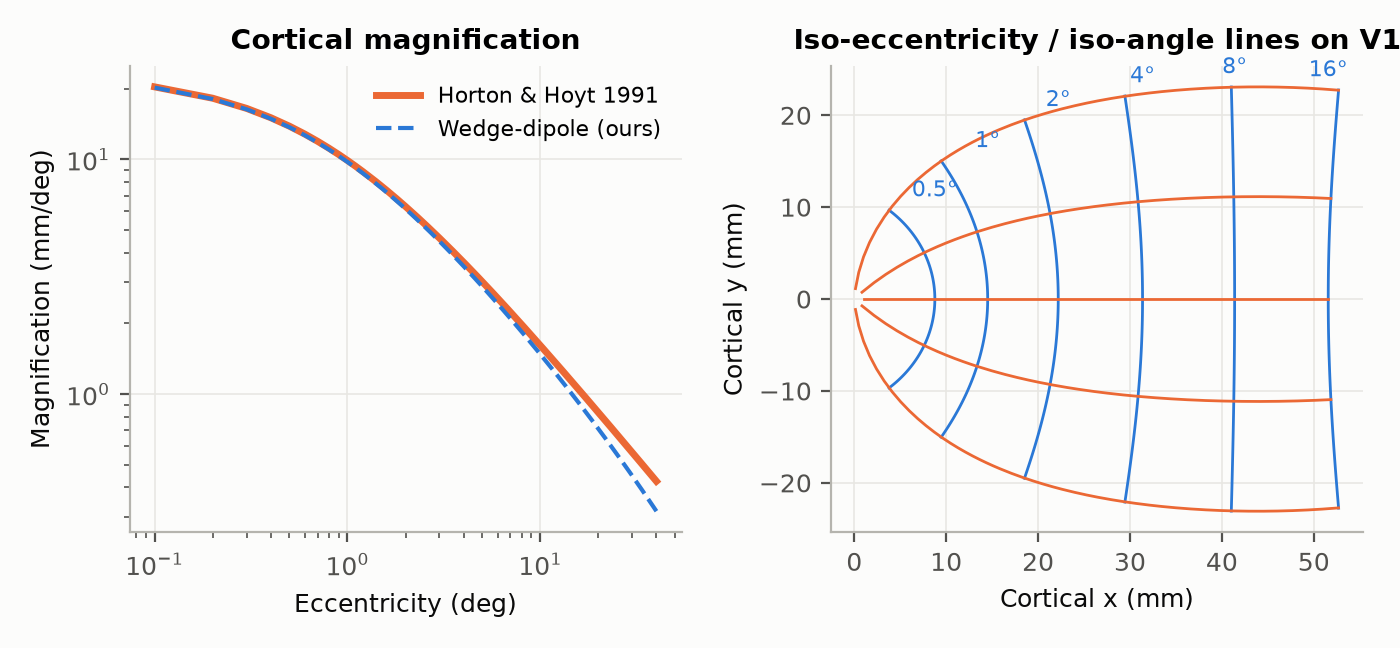
\includegraphics[width=0.49\textwidth]{fig_sim_magnification.png}\hfill
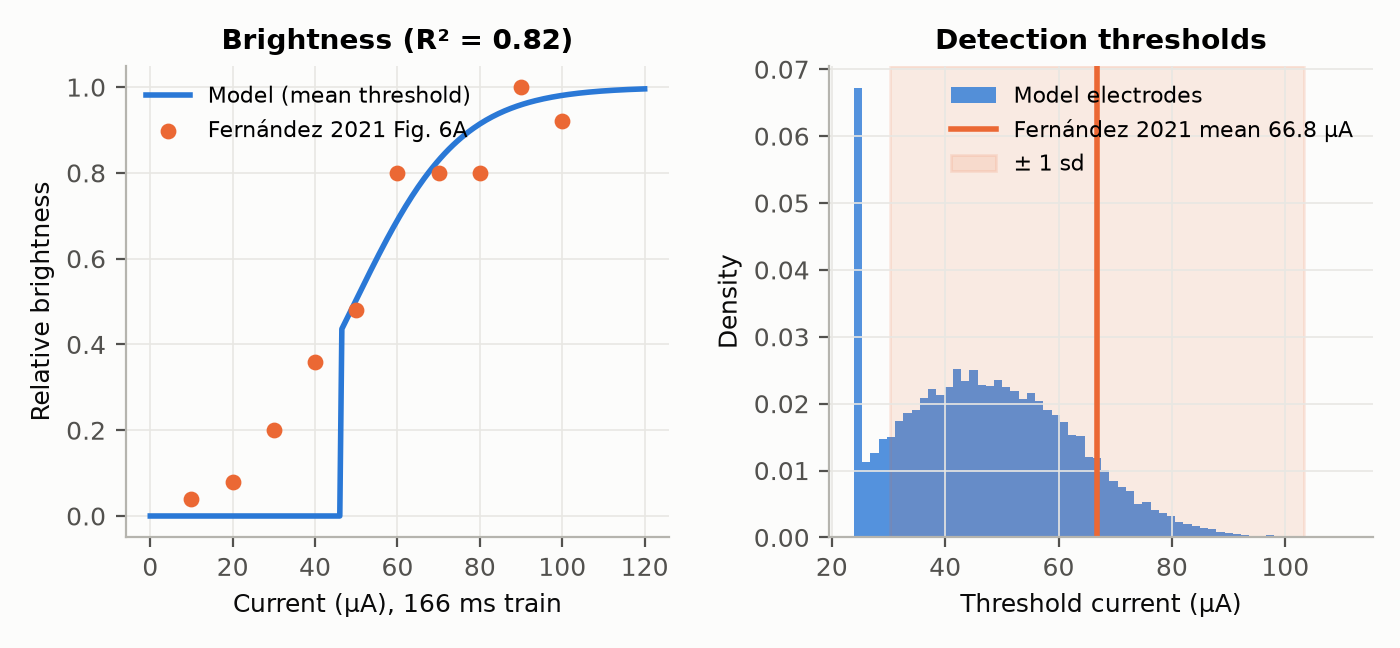
\includegraphics[width=0.49\textwidth]{fig_sim_brightness_threshold.png}\\[2pt]
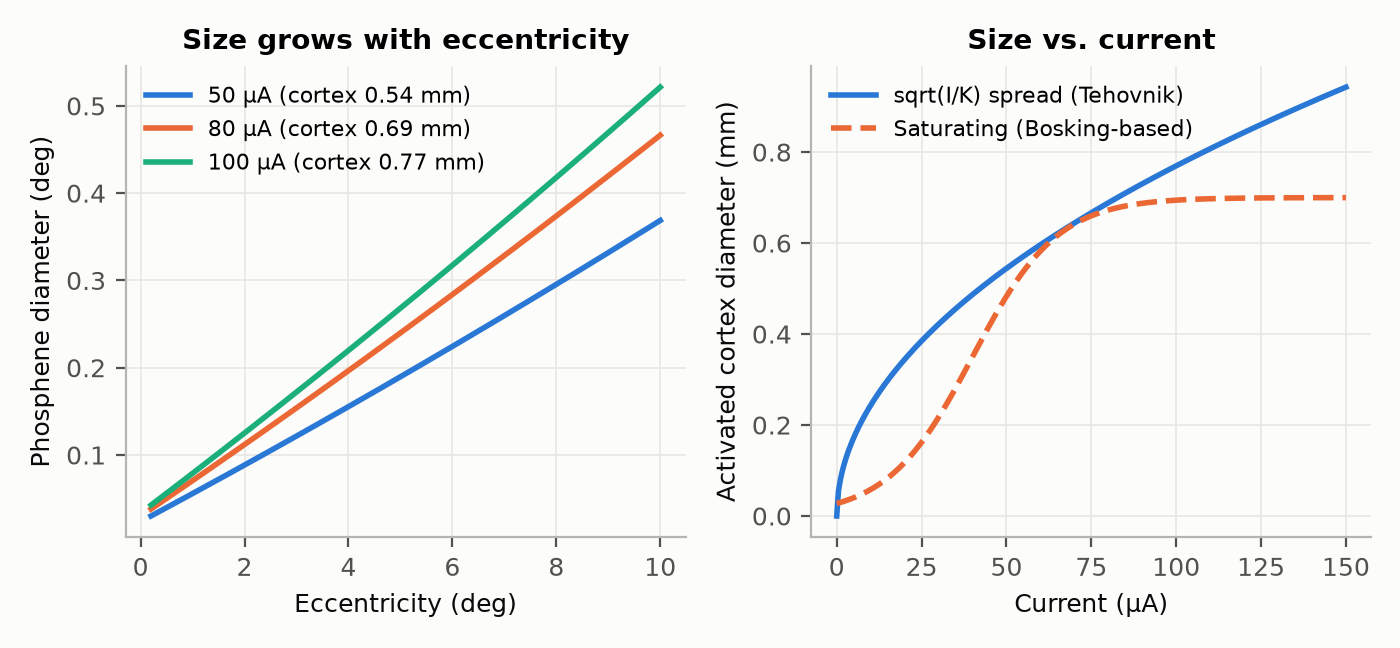
\includegraphics[width=0.49\textwidth]{fig_sim_size.png}\hfill
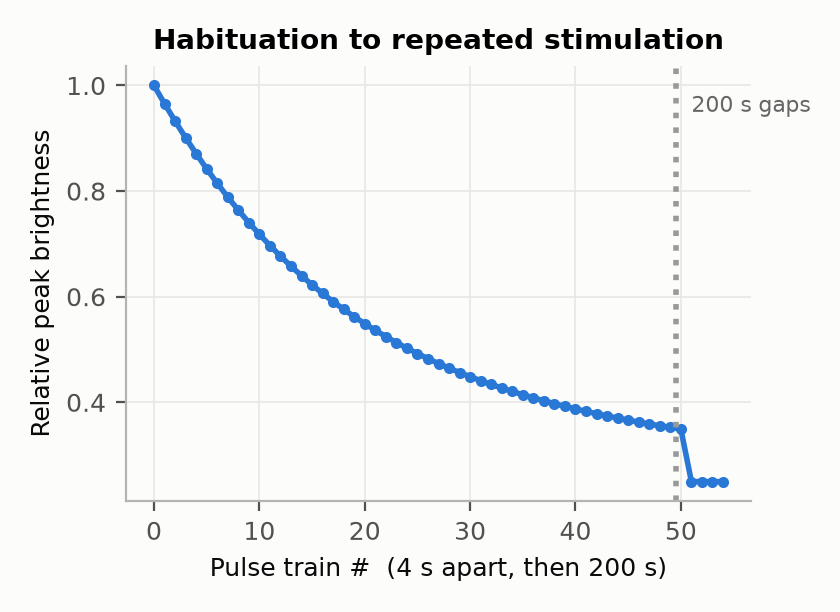
\includegraphics[width=0.30\textwidth]{fig_sim_habituation.png}\hspace*{0.1\textwidth}
\caption{Simulator validation.
\textbf{Top left:} wedge-dipole magnification against \citet{horton1991representation}, and the cortical map.
\textbf{Top right:} brightness against current compared with \citet{fernandez2021visual} Fig.~6A; threshold distribution compared with their reported mean $\pm$ s.d.
\textbf{Bottom:} phosphene size against eccentricity and current, including the saturating Bosking-based alternative; habituation under repeated trains.}
\label{fig:sim}
\end{figure*}

\begin{figure*}[t]
\centering
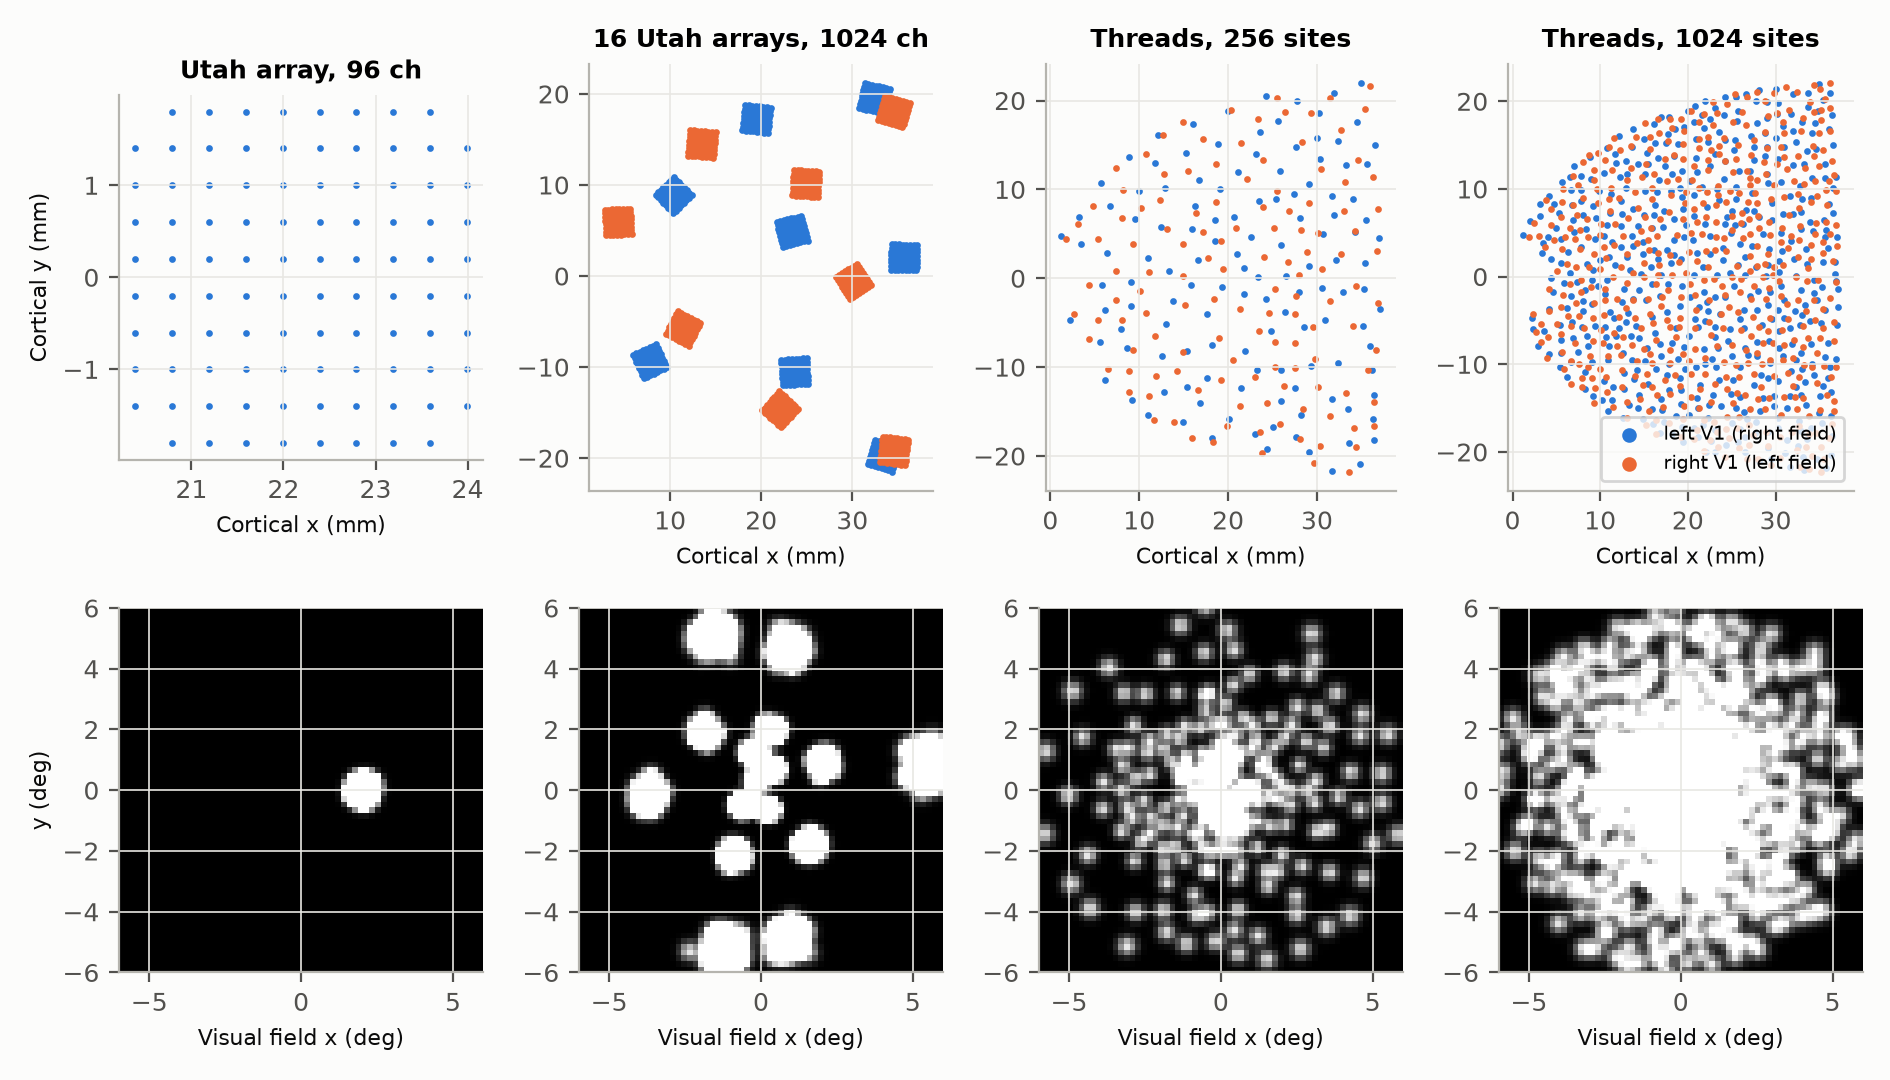
\includegraphics[width=0.85\textwidth]{fig_sim_layouts.png}
\caption{Electrode layouts on the flattened cortex (top row; blue = left V1, orange = right V1) and the percept of all electrodes at 80\,\textmu A for a held-out patient (bottom row).}
\label{fig:layouts}
\end{figure*}

\section{Stimulus encoders}\label{sec:enc}
Every encoder maps a $64{\times}64$ grayscale image spanning the $12^\circ$ field to amplitudes $a\in\mathbb R^N$. The amplitudes pass through a shared \textbf{safety layer} that clamps to $[0, I_{\max}{=}100\,\text{\textmu A}]$ (17\,nC/phase at 170\,\textmu s) and keeps at most $k{=}\lceil 0.25N\rceil$ active electrodes per frame. These stand in for charge-density and power/crosstalk budgets \citep{shannon1992model,cogan2008neural}.

\paragraph{Baselines.} All baselines sample a feature map bilinearly at each nominal phosphene centre. A sampled value $v_n\in[0,1]$ maps linearly from the electrode's (calibrated) threshold current to $I_{\max}$, and values $v_n\le0.1$ give zero current. The baselines are:
\begin{itemize}
\item \textbf{Intensity}: Gaussian-blurred image ($\sigma{=}1$\,px), in an \emph{uncalibrated} version (mean threshold, all electrodes assumed alive) and a \emph{calibrated} version;
\item \textbf{Edges}: Sobel magnitude;
\item \textbf{Salient edges}: Sobel magnitude weighted by spectral-residual saliency \citep{hou2007saliency}, a light-weight scene simplification \citep{han2021deep};
\item \textbf{Per-image optimisation}: for reference, amplitudes optimised separately for every image through the true patient simulator (100 Adam steps). This is non-causal and far too slow for real-time use.
\end{itemize}

\paragraph{Learned encoder.} The architecture has three stages:
\begin{enumerate}
\item A small U-Net (input image plus $x$, $y$ and eccentricity coordinate channels; resolutions 32 and 16; width 24) produces a stimulation map $s$ at half resolution.
\item The map is read out bilinearly at the nominal phosphene centres, $u_n=s(x_n,y_n)$.
\item The amplitude is $a_n=I_{\max}\,\mathrm{sigmoid}(g_n u_n+\beta_n)$.
\end{enumerate}
The network has \NumEncParams\ parameters for 1024 electrodes, because only the per-electrode gain and bias $(g_n,\beta_n)$ grow with $N$. The read-out uses only Gather operations, so the encoder exports to ONNX for in-browser and on-device inference.

\paragraph{Objective.} A decoder $D$ (a small CNN) reconstructs the image from the percept. With $\Phi=\mathcal S(\mathrm{Safety}(E(x));\text{patient})$:
\begin{multline}
\mathcal L = \|D(\Phi)-x\|^2 + \|\Phi-x\|^2 \\ + 0.5\,(1-\mathrm{SSIM}(\Phi,x)) + 0.05\,\overline{a/I_{\max}}.
\end{multline}
\begin{itemize}
\item The reconstruction term \citep{deruyter2022end} keeps the percept informative.
\item The percept terms keep it directly interpretable, since a person has no decoder.
\item The charge term discourages unnecessary stimulation.
\end{itemize}
We train with domain randomisation: the patient switches every 20 steps among 16 training patients that are disjoint from the test patients.

\paragraph{Patient adaptation.} After implantation, threshold mapping gives a calibrated forward model of that patient. We fine-tune a copy of the generic encoder for each patient, updating only the adapter $(g,\beta)$ (2$N$ parameters, decoder frozen). This uses 256 unlabeled images and 150 Adam steps. No labels or behavioural data are needed. We also compare against full fine-tuning with 16 to 1024 images.

\section{Experimental setup}
\begin{itemize}
\item \textbf{Data.} MNIST digits, EMNIST letters (26 classes; \citealp{cohen2017emnist}) and grayscale CIFAR-10 as a small natural-image proxy. Images are resized to $64{\times}64$ and fill the $12^\circ$ field.
\item \textbf{Training.} Encoders are trained on 20k training images for 1500 steps at batch size 32, with three seeds per dataset.
\item \textbf{Patients.} Evaluation uses five held-out patients (seeds 1000--1004) on the threads-1024 layout. Images are assigned to patients round-robin.
\item \textbf{Metrics.}
  \begin{itemize}
  \item SSIM \citep{wang2004image} and PSNR between percept and input.
  \item \emph{Low-pass SSIM}, computed after blurring both images with $\sigma{=}0.375^\circ$. Phosphene vision cannot carry detail finer than the phosphene spacing, and raw SSIM mostly scores dot texture.
  \item \emph{Recognition accuracy}: a fresh CNN is trained on each encoder's percepts of 6k training images (4 epochs) and tested on 2k test images. It stands in for a user who has learned that encoding \citep{rassia2018improvement}; the same CNN on the original images gives a ceiling.
  \item Stimulation cost: active electrodes per frame and summed charge per phase.
  \item Robustness: additional unannounced electrode failures (10/25/50\%), with no recalibration or retraining.
  \end{itemize}
\item \textbf{Compute.} Everything runs on a shared 8-core Intel CPU with 2 threads per process. A training run takes about \NumTrainMin\ minutes.
\end{itemize}

\section{Results}\label{sec:results}
\GenMainTable

\paragraph{Main comparison.} Table~\ref{tab:main} and Fig.~\ref{fig:main} give the results; Fig.~\ref{fig:examples} shows examples. On all three datasets the learned encoder beats every causal baseline on SSIM, low-pass SSIM and PSNR, and uses less charge than the calibrated intensity baseline:
\begin{itemize}
\item \textbf{Letters.} Low-pass SSIM is \NumLettersLearnLp\ against \NumLettersIntLp. Accuracy is \NumLettersLearnAcc\ against \NumLettersIntAcc, which is on par with the same classifier on the original images (\NumLettersCeil).
\item \textbf{MNIST.} Every reasonable encoder gets near the ceiling (\NumMnistLearnAcc\ against \NumMnistIntAcc, ceiling \NumMnistCeil), so 1024 well-spread sites carry digits easily. Image fidelity still separates the encoders: low-pass SSIM is \NumMnistLearnLp\ against \NumMnistIntLp.
\item \textbf{CIFAR-10.} The ceiling is low because grayscale 32\,px objects are hard even unprosthetised (\NumCifarCeil). The learned encoder raises accuracy from \NumCifarIntAcc\ to \NumCifarLearnAcc\ and low-pass SSIM from \NumCifarIntLp\ to \NumCifarLearnLp.
\item \textbf{Charge.} The learned encoder uses \NumMnistLearnCharge\ against \NumMnistIntCharge\,\textmu C of summed charge per phase on MNIST, and \NumLettersLearnCharge\ against \NumLettersIntCharge\ on letters.
\end{itemize}
The two edge-based encoders score poorly on image similarity by construction, since they render outlines of filled shapes. They are also below intensity sampling on recognition here. Scene simplification aimed at navigation \citep{han2021deep} needs semantic segmentation, which our light saliency proxy does not provide.

\paragraph{Amortised versus per-image optimisation.} Per-image optimisation knows the true patient and optimises each frame separately, evaluated on the first 128 test images per patient. On MNIST and letters it is only marginally better than the single-pass learned encoder (SSIM \NumMnistOracleSsim\ against \NumMnistLearnSsim; \NumLettersOracleSsim\ against \NumLettersLearnSsim). On CIFAR it is clearly better (\NumCifarOracleSsim\ against \NumCifarLearnSsim), which leaves headroom for larger encoders on natural images. It also stimulates fewer electrodes (\NumMnistOracleActive\ against \NumMnistLearnActive\ on MNIST). With 100 Adam steps through the fast renderer it is a reference point, not an upper bound.

\paragraph{Patient adaptation.} Fine-tuning only the per-electrode gain and bias on a patient's calibrated forward model raised SSIM on every dataset:
\begin{itemize}
\item MNIST: \NumMnistLearnSsim\,$\to$\,\NumMnistAdaptSsim;
\item letters: \NumLettersLearnSsim\,$\to$\,\NumLettersAdaptSsim;
\item CIFAR: \NumCifarLearnSsim\,$\to$\,\NumCifarAdaptSsim;
\item CIFAR low-pass SSIM: \NumCifarLearnLp\,$\to$\,\NumCifarAdaptLp.
\end{itemize}
Recognition changed little: MNIST \NumMnistLearnAcc\,$\to$\,\NumMnistAdaptAcc, letters \NumLettersLearnAcc\,$\to$\,\NumLettersAdaptAcc, CIFAR \NumCifarLearnAcc\,$\to$\,\NumCifarAdaptAcc. The generic encoder knows neither thresholds nor dead electrodes, and only \NumMnistLearnSupraPct\% of the currents it delivers on MNIST exceed the patient's detection threshold. Calibrated intensity sampling puts \NumMnistIntSupraPct\% above threshold. The adapter did not raise this share (\NumMnistAdaptSupraPct\%). Instead it used more of the active-electrode budget (\NumMnistAdaptActive\ against \NumMnistLearnActive\ active electrodes) at a lower median current (\NumMnistAdaptMedAmp\ against \NumMnistLearnMedAmp\,\textmu A), i.e.\ more but dimmer and smaller phosphenes. Figure~\ref{fig:adapt} shows how the gain depends on the number of unlabeled images (MNIST, two patients). Sixteen images give no reliable gain (\NumShotAdptA\ SSIM). The adapter's gain grows to \NumShotAdptD\ with 1024 images, while full fine-tuning at the same step budget levels off near \NumShotFullC. At this step budget, restricting adaptation to the per-electrode parameters is both cheaper and more effective.

\begin{figure*}[t]
\centering
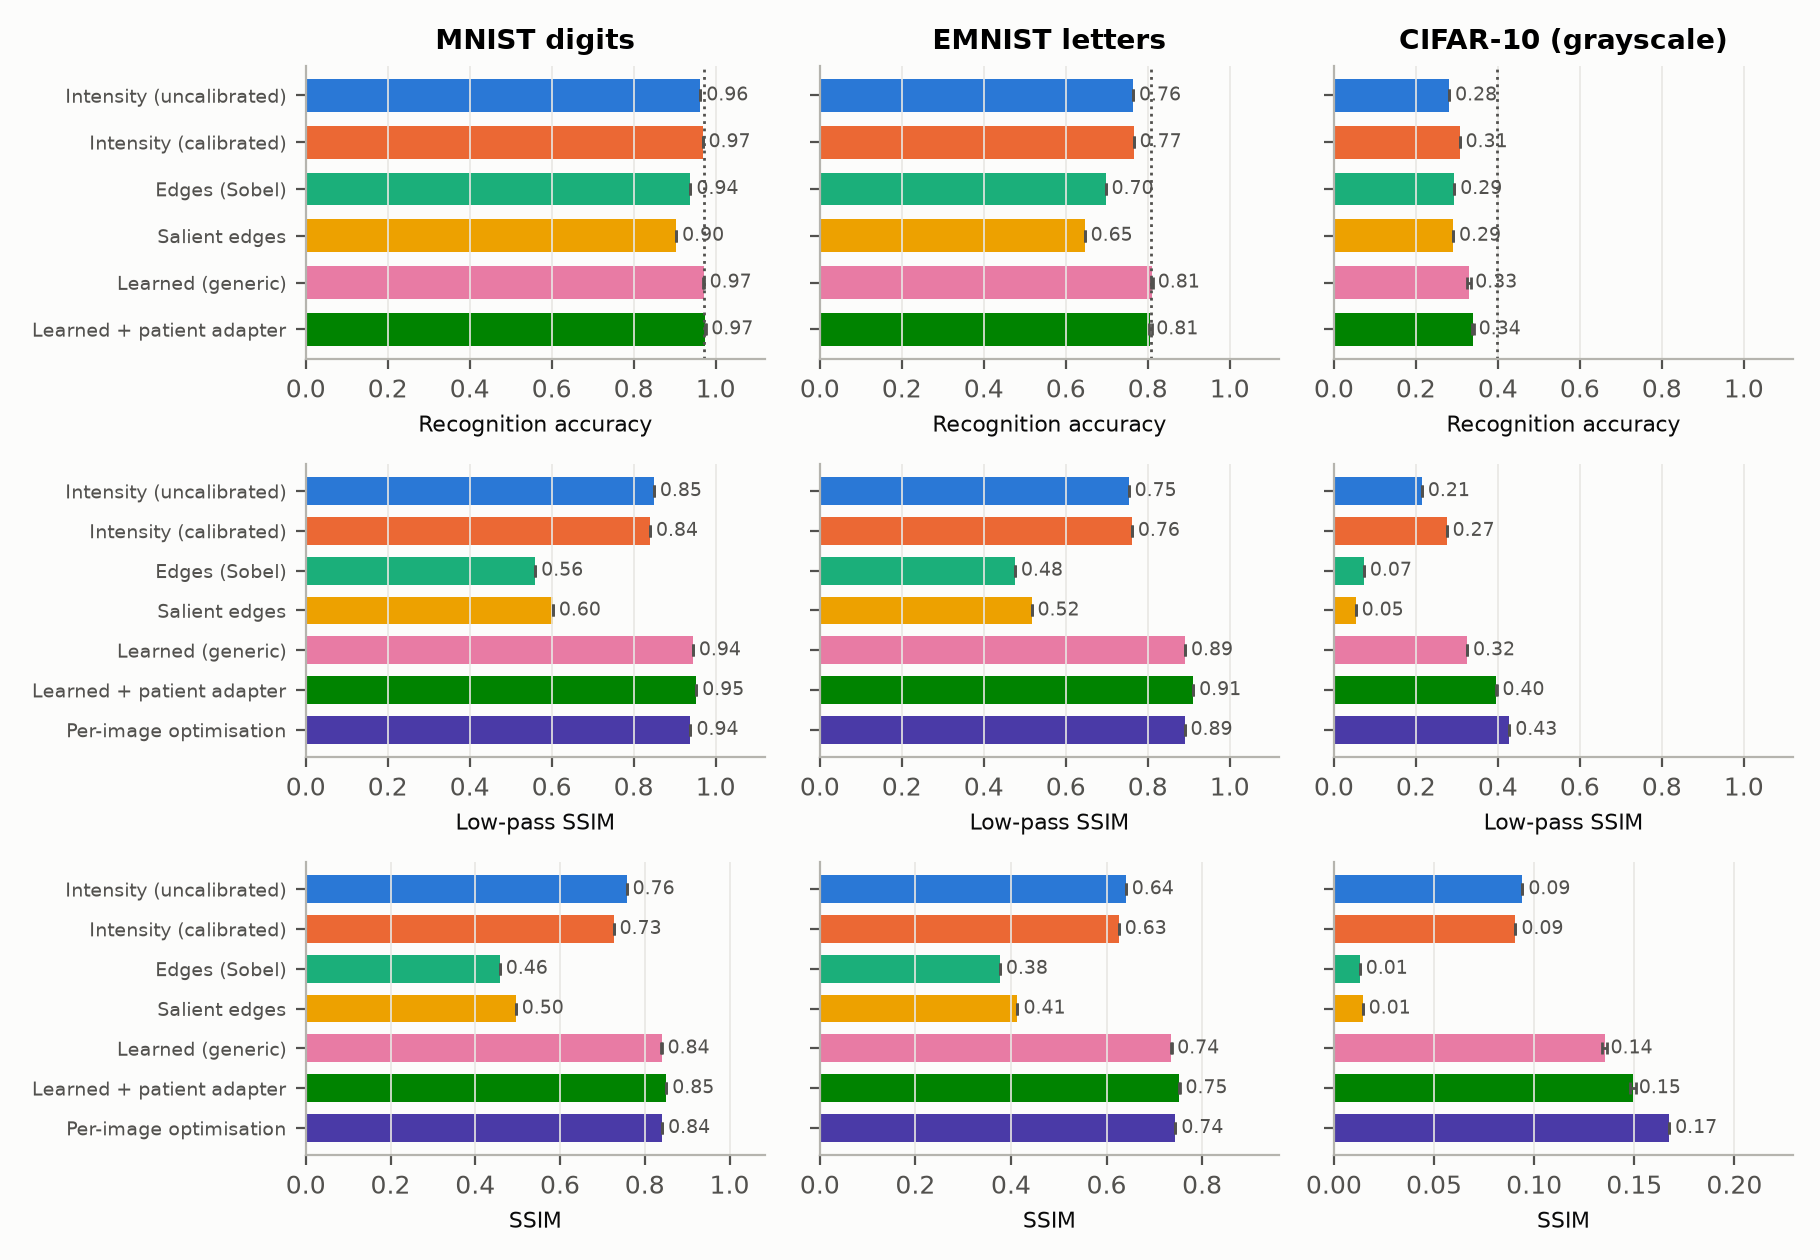
\includegraphics[width=\textwidth]{fig_main_results.png}
\caption{Main results per dataset (five held-out patients; learned rows show mean and s.d.\ over three training seeds). The dotted line marks the classifier's accuracy on the original images.}
\label{fig:main}
\end{figure*}

\begin{figure}[t]
\centering
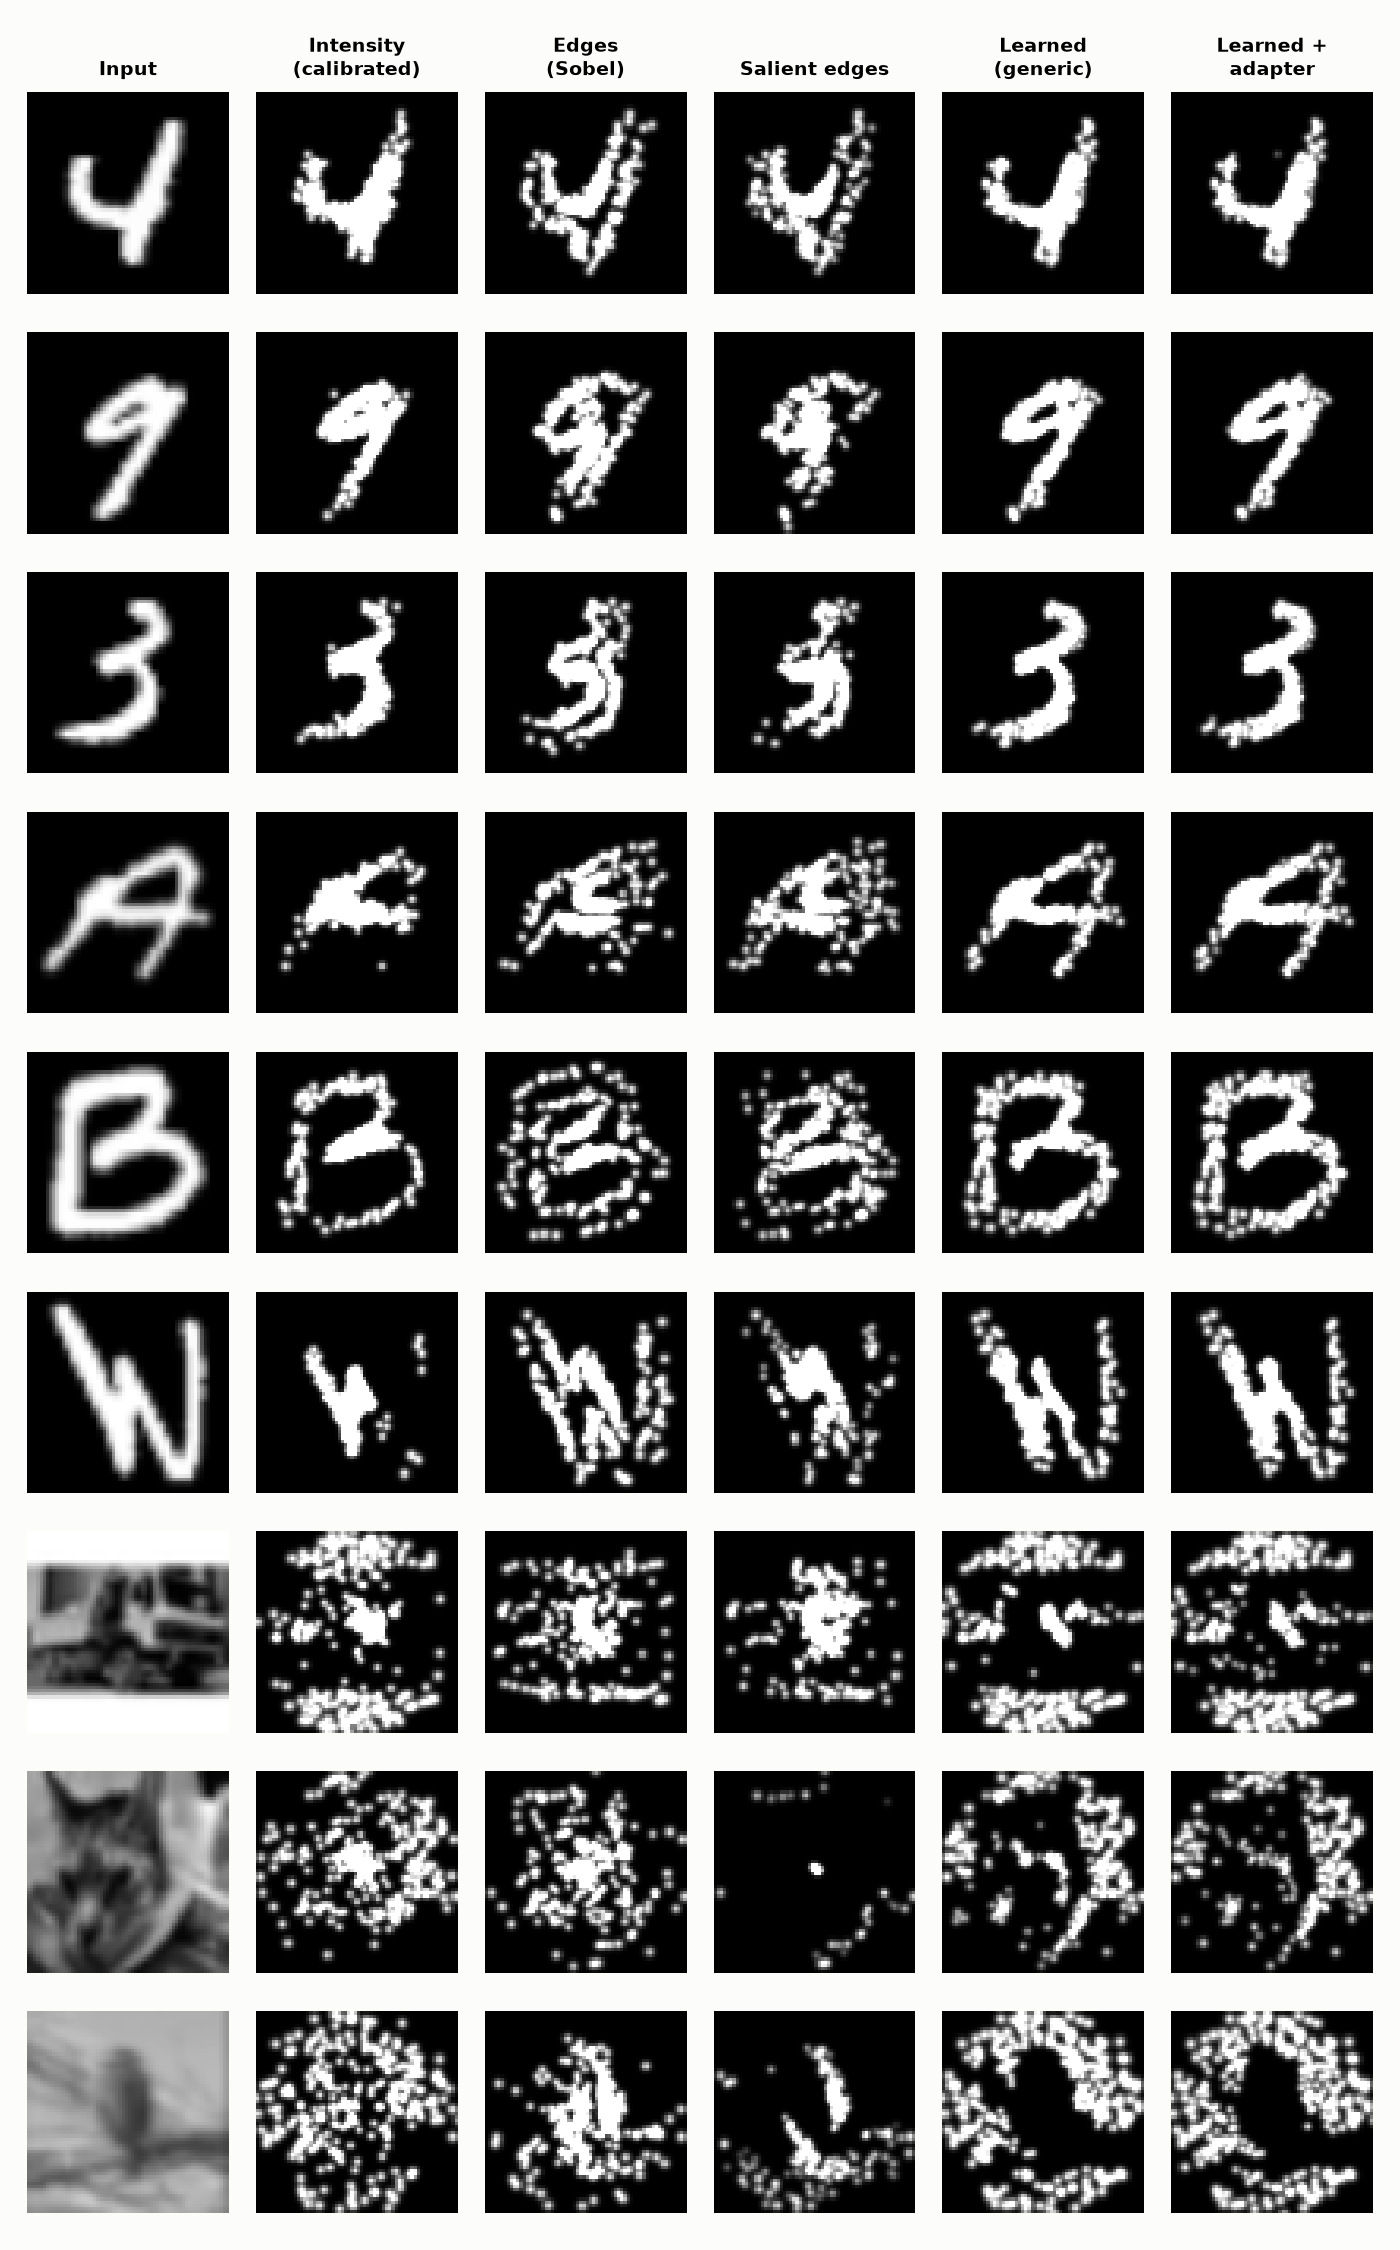
\includegraphics[width=\columnwidth]{fig_examples.png}
\caption{Example percepts on held-out patients for MNIST, EMNIST letters and CIFAR-10. With a 25\% active-electrode budget, intensity sampling can only light the 256 brightest sites, and drops parts of large shapes (e.g.\ the ``W''). The learned encoder spreads the same budget along the strokes.}
\label{fig:examples}
\end{figure}

\paragraph{Robustness to electrode failure.} Table~\ref{tab:dropout} and Fig.~\ref{fig:dropout} show performance after up to 50\% of the remaining electrodes fail without warning, with no recalibration and no classifier retraining:
\begin{itemize}
\item All encoders degrade gracefully up to 25\%.
\item At 50\% on MNIST and letters the learned encoder stays at or above the intensity baseline (\NumLettersLearnAccDropHalf\ against \NumLettersIntAccDropHalf\ on letters).
\item On CIFAR at 50\% it falls \emph{below} intensity sampling (\NumCifarLearnAccDropHalf\ against \NumCifarIntAccDropHalf).
\end{itemize}
Our reading of the CIFAR result is that the end-to-end encoder learns a distributed, texture-like code. That code is more informative when intact, but its percepts change more when half of it disappears, and the classifier was trained on intact percepts. Training-time electrode dropout beyond the 10\% in the training patients is the obvious fix, which we leave to the full-scale runs.

\GenDropoutTable

\begin{figure*}[t]
\centering
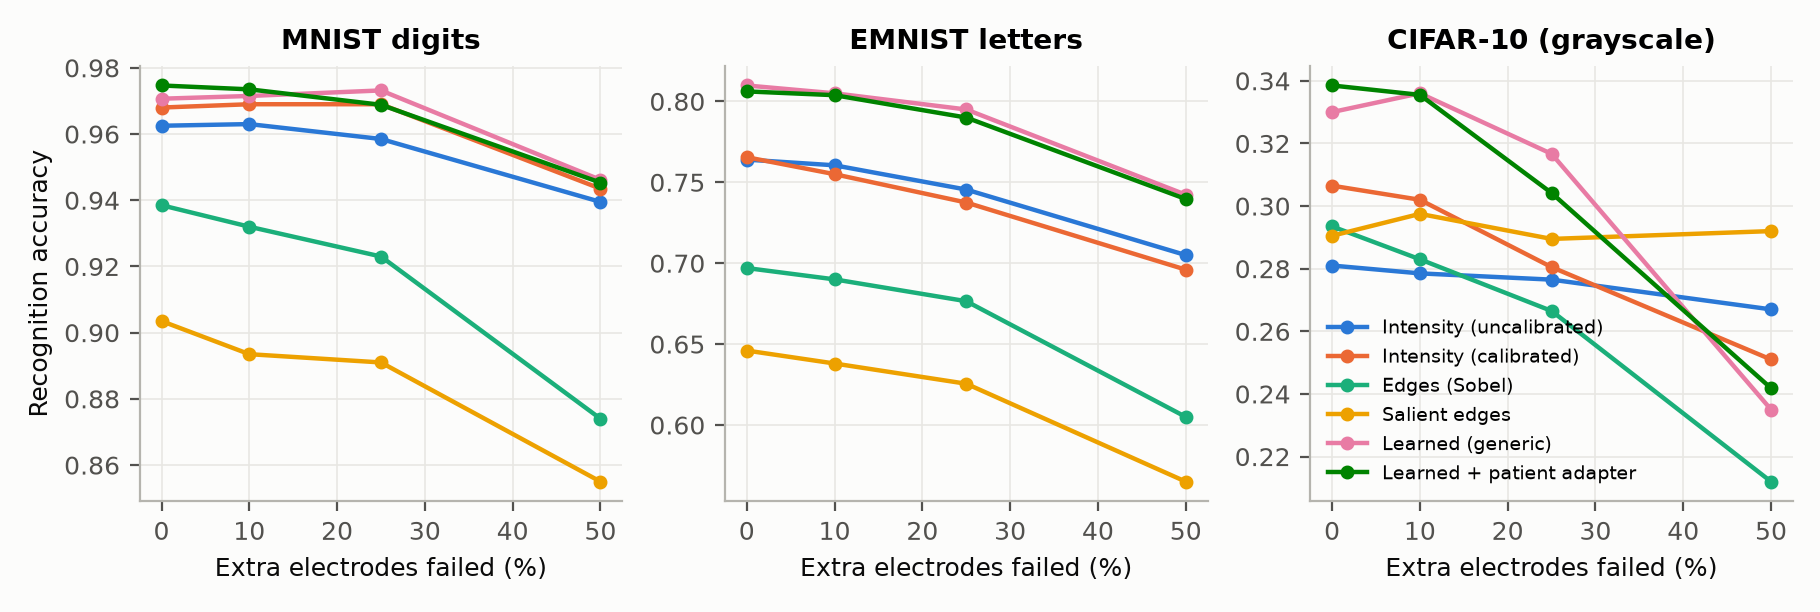
\includegraphics[width=\textwidth]{fig_dropout_robustness.png}
\caption{Recognition accuracy against the fraction of additional, unannounced electrode failures.}
\label{fig:dropout}
\end{figure*}

\section{Ablations}\label{sec:ablation}
\GenAblationTable
\paragraph{Loss terms.} Table~\ref{tab:ablation} (upper block) varies the training objective on MNIST.
\begin{itemize}
\item \textbf{Percept-similarity term is essential.} Without it, training collapsed within the first 300 steps to currents below the rheobase, i.e.\ no phosphenes. The result is SSIM \AbNoPerSsim\ and accuracy \AbNoPerAcc, with a charge of essentially zero. With the decoder loss as the only objective, the gradient reaching a dark electrode passes through the sub-rheobase ReLU and the narrow threshold surrogate. Once most electrodes fall below threshold, that gradient vanishes.
\item \textbf{Decoder loss did not help at this scale.} Dropping it gave SSIM \AbNoRecSsim\ and accuracy \AbNoRecAcc, against \AbMainSsim\ and \AbMainAcc\ for the full objective.
\item \textbf{Charge cost is cheap.} Removing it raised summed charge from \AbMainCharge\ to \AbNoChgCharge\,\textmu C per phase without improving fidelity (SSIM \AbNoChgSsim).
\end{itemize}

\paragraph{Safety limits.} Removing the active-electrode cap and the charge cost, and raising the ceiling to 200\,\textmu A, gives better images: SSIM \AbUnconSsim\ against \AbMainSsim. The price is \AbUnconActive\ active electrodes instead of \AbMainActive\ and \AbUnconCharge\ against \AbMainCharge\,\textmu C of charge per phase, while recognition is unchanged (\AbUnconAcc\ against \AbMainAcc). For a device that must manage charge, heat and power, the constrained operating point is clearly preferable.

\paragraph{Electrode count and layout.} The lower block of Table~\ref{tab:ablation} and Fig.~\ref{fig:ablation} vary the implant.
\begin{itemize}
\item \textbf{Threads.} With 64 and 256 sites the learned encoder still beats intensity sampling on recognition: \AbThrAAcc\ against \AbThrAIntAcc, and \AbThrBAcc\ against \AbThrBIntAcc. Its relative advantage is largest when phosphenes are scarce.
\item \textbf{One Utah array (96 channels).} It covers only a $\sim$0.6$^\circ$ patch near $2^\circ$ eccentricity, so neither encoder can convey digits (accuracy \AbUtahAAcc\ learned, \AbUtahAIntAcc\ intensity). End-to-end training here also collapsed to no stimulation: the charge fell to essentially zero within 300 steps, the same dead-zone failure as above.
\item \textbf{Sixteen Utah arrays (1024 contacts).} They reach \AbUtahBAcc\ (learned) and \AbUtahBIntAcc\ (intensity); here intensity sampling is slightly better. Both are well below the same number of thread sites (\AbMainAcc), because the contacts cluster into 16 small patches of the visual field, where neighbouring phosphenes overlap.
\end{itemize}

\begin{figure}[t]
\centering
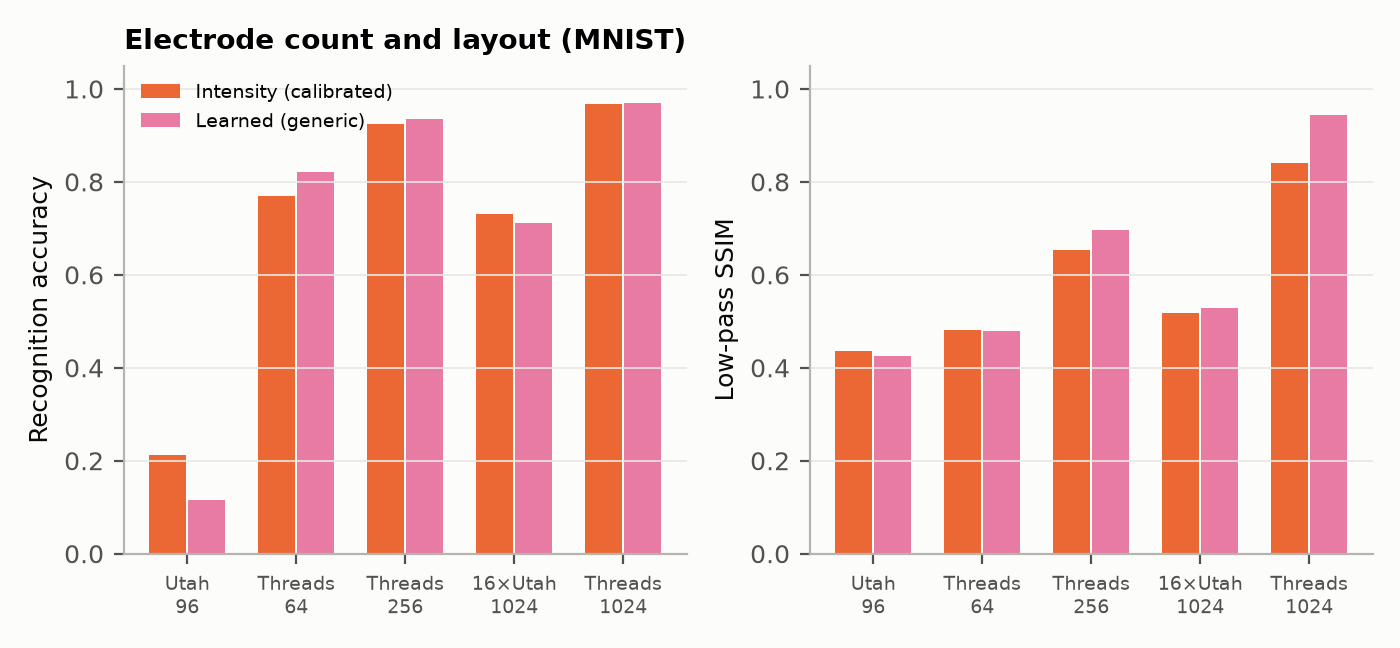
\includegraphics[width=\columnwidth]{fig_ablation_layouts.png}\\[2pt]
\IfFileExists{../results/figures/fig_adaptation_shots.png}{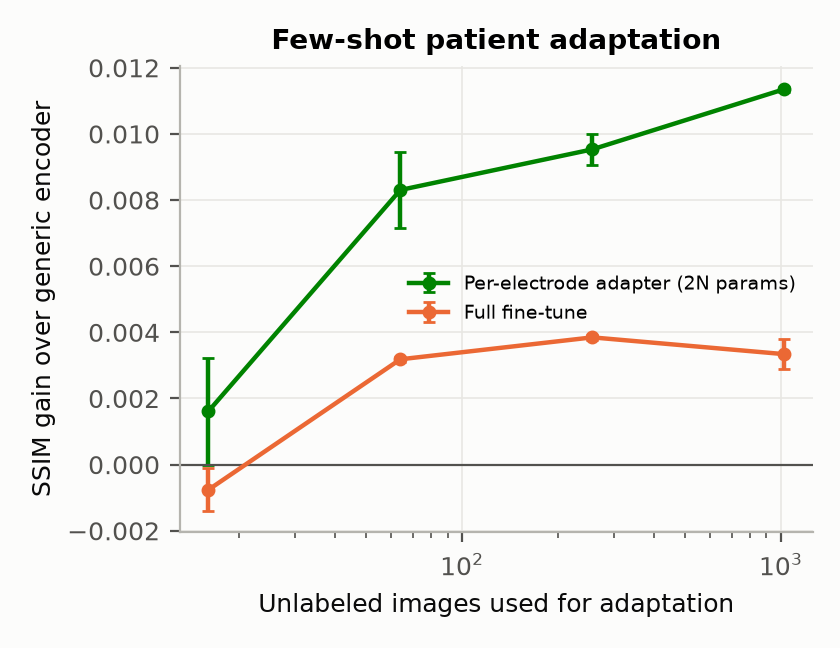
\includegraphics[width=0.75\columnwidth]{fig_adaptation_shots.png}}{}
\caption{\textbf{Top:} recognition and low-pass SSIM against electrode layout (MNIST, seed 0), learned encoder against intensity sampling. \textbf{Bottom:} SSIM gain from patient adaptation against the number of unlabeled images. MNIST, two held-out patients, 150 steps. With 64 or more images, adapter-only fine-tuning (2$N$ parameters) gains more than full fine-tuning.}
\label{fig:ablation}\label{fig:adapt}
\end{figure}


\section{Discussion}
\paragraph{What the learned encoder learns.} Three observations follow from Fig.~\ref{fig:examples} and from the budget diagnostics (\texttt{results/eval/diagnostics.json}):
\begin{itemize}
\item \textbf{Budget allocation.} Intensity sampling fills its 25\% active-electrode budget with whichever sites are brightest, and can drop whole parts of a shape (the ``W''). The learned encoder activates fewer sites (\NumMnistLearnActive\ against \NumMnistIntActive\ on MNIST) but keeps strokes continuous.
\item \textbf{Thresholds.} The generic encoder does not know the patient's thresholds, and \NumMnistLearnSupraPct--\NumCifarLearnSupraPct\% of its delivered currents exceed them (MNIST to CIFAR). The calibrated baseline reaches \NumMnistIntSupraPct\% on MNIST. Wasted sub-threshold stimulation is therefore a remaining inefficiency that a threshold-aware adapter or a threshold input channel could remove.
\item \textbf{Natural images.} With only $\sim$250 phosphenes the learned encoder renders coarse luminance layout and large contours rather than texture, which resembles a learned scene simplification. This is where low-pass SSIM rises most (\NumCifarIntLp\ to \NumCifarAdaptLp).
\end{itemize}

\paragraph{Why a retinotopic read-out.} A dense output layer for 1024 electrodes would hold most of the model's parameters, would be tied to one electrode layout, and could not use the fact that nearby phosphenes should get similar commands. Our convolutional map with a bilinear read-out avoids all three problems:
\begin{itemize}
\item it has \NumEncParams\ parameters in total;
\item the read-out positions are a buffer, not learned weights, so the trunk is not tied to one layout (we did not test transfer between layouts);
\item all per-person variation sits in a 2$N$-parameter adapter.
\end{itemize}
This split fits the clinical workflow. A generic model is trained once in simulation. Each patient's adapter is then fitted to that person's mapping data: thresholds and dead electrodes now, phosphene locations once mapped. If no calibrated forward model is available, the adapter's low dimension makes it a natural target for preference-based optimisation \citep{granley2023human}.

\paragraph{Implications for implant design.} The layout ablation separates electrode \emph{count} from \emph{coverage}. One Utah array covers \NumCovUtahNine\% of the central field, so neither encoder conveys digits with it (accuracy at most \AbUtahAIntAcc). Sixteen arrays with 1024 contacts cover \NumCovUtahThou\%, because each 3\,mm array lands on one small patch of the field. The same number of independently placed thread sites covers \NumCovThrThou\%. Under our assumptions, a 1024-channel device gains most from spreading its insertion sites over the reachable cortex. Packing more contacts into rigid grids helps far less.

\section{Limitations}\label{sec:limits}
\begin{itemize}
\item \textbf{Simulation only.} Every result depends on the phosphene model. That model is fitted to one human Utah-array study \citep{fernandez2021visual}, a few earlier reports, and parameters some of which the dynaphos authors describe as not fitted to data (e.g.\ $\tau_{\mathrm{act}}$).
  \begin{itemize}
  \item Our threshold distribution has mean \NumThrMean\,\textmu A, lower than the 66.8\,\textmu A reported by Fernández et al.
  \item The model leaves out phosphene shape, colour and flicker; interactions between electrodes (current summation, threshold reduction under simultaneous stimulation, which Fernández et al.\ observed); and gaze-contingent shifts of phosphene location.
  \end{itemize}
\item \textbf{Planar cortex.} The thread layout assumes uniformly reachable V1 on a plane. Much of real V1 lies inside the calcarine sulcus, so coverage is optimistic. The layout is our idealisation, not a device specification.
\item \textbf{Static frames.} We optimise single 166\,ms frames. Temporal encoding (dynamic current steering, \citealp{beauchamp2020dynamic}) and managing habituation over seconds are not addressed, although the simulator models habituation.
\item \textbf{Recognition proxy.} A CNN trained on percepts upper-bounds what a person could learn: it has unlimited training, no attention limits and no fatigue. Human psychophysics with simulated prosthetic vision would be the next validation step.
\item \textbf{Scale.} Networks are small, data are low-resolution benchmarks, training is 1500 steps, and patients are few. Standard deviations over three seeds are small, but conclusions about natural scenes (CIFAR) in particular are preliminary.
\item \textbf{Two training failures.}
  \begin{itemize}
  \item With a single 96-channel array, end-to-end training collapsed to no stimulation (discussed above).
  \item Without safety limits, a first run that initialised every electrode at 100\,\textmu A also collapsed. Its training log (\texttt{results/extra\_runs/}) shows the charge term going to zero. The reported unconstrained variant starts at 50\,\textmu A like every other run.
  \end{itemize}
  Both point to dead zones (sub-rheobase currents and saturated sigmoids) as a practical pitfall of end-to-end stimulation learning.
\end{itemize}

\section{Broader impact and safety}
The stimulus encoder is the software that decides how much current enters a person's brain, so it is safety-critical. Our design keeps safety outside the learned component:
\begin{itemize}
\item the same hard clamp and active-electrode cap apply to every encoder, learned or not;
\item the learned model can only choose \emph{within} the safe set.
\end{itemize}
A deployable system would also need charge-density limits specific to the electrode material and geometry \citep{shannon1992model,cogan2008neural}, limits on cumulative charge over time, monitoring for threshold drift, and clinician-set per-electrode ceilings. Our numbers are not a statement about any real device's safety.

Simulated recognition rates must not be read as predictions of what a blind person will see. Communicating that uncertainty honestly matters, because expectations for these devices are high. This is an independent project, not affiliated with or endorsed by Neuralink, and it uses no proprietary data.

\section{Reproducing at full scale}\label{sec:repro}
Everything above comes from \texttt{scripts/run\_cpu.sh} (\texttt{configs/cpu.yaml}). That script runs the pipeline end to end: data, simulator validation, training, evaluation, ablations, adaptation, figures and website export, followed by the unit tests.

\texttt{scripts/run\_gpu.sh} runs the same code with \texttt{configs/gpu.yaml} on a CUDA machine. The device is detected automatically; the CNNs run under bfloat16 autocast and the simulator in float32. It scales up:
\begin{itemize}
\item training: 20k steps at batch size 128, 100k training images, network width 48;
\item seeds and patients: five seeds, 64 training patients, ten test patients;
\item evaluation: 50k classifier images, 300-step per-image optimisation, three ablation seeds, and a 2048-site layout.
\end{itemize}
The script creates its own virtual environment from \texttt{requirements-gpu.txt} and downloads the datasets. The figures, \texttt{metrics.json} and these tables are regenerated from its outputs by \texttt{paper/make\_tables.py}.


\bibliographystyle{unsrtnat}
\bibliography{refs}
\end{document}
